
\documentclass{beamer}
% Load Packages
\usepackage[utf8]{inputenc}
\usepackage{xcolor}
\usepackage{tikz}
\usetikzlibrary{positioning,calc}
\usepackage{graphicx}
\usepackage{hyperref}
\usepackage{amsmath}
\usepackage{listings}
\usepackage{fontawesome}

% Define Commands
\newcommand*{\ClipSep}{0.06cm} %To adjust footer logo
\newcommand{\E}{\mathrm{e}\,} %\def\I{e} % used to defined e for exp(x), see later what it should be
\newcommand{\ud}{\mathrm{d}}
\lstset{numbers=left, numberstyle=\tiny, stepnumber=1,firstnumber=1,breaklines=true,
    numbersep=5pt,language=Python,
    stringstyle=\ttfamily,
    basicstyle=\footnotesize, 
    showstringspaces=false
}

\usetheme{oxonian}

\title{Hold Your Tongue!: Sentiment Analysis and Classification in the Legal Field}
\titlegraphic{
\includegraphics[width=4.8cm]{Theme/Logos/ousigil.png}}
\author{Sloan C. Stinnett}
\institute{University of Oklahome}
\date{April 2019} %\today

\usepackage[utf8]{inputenc}
\usepackage[authoryear]{natbib}
\usepackage{graphicx}

\begin{document}

{\setbeamertemplate{footline}{} 
\frame{\titlepage}}

\section*{Outline}\begin{frame}{Outline}\tableofcontents\end{frame}

\section{Introduction}
    \begin{frame}[plain]
        \vfill
      \centering
      \begin{beamercolorbox}[sep=8pt,center,shadow=true,rounded=true]{title}
        \usebeamerfont{title}\insertsectionhead\par%
        \color{oxfordblue}\noindent\rule{10cm}{1pt} \\
      \end{beamercolorbox}
      \vfill
  \end{frame}
  
\subsection{Introduction}
\begin{frame}{Introduction}
\begin{itemize}
    \item  Rhetoric has a deep historical connection with law.
    \item Psychologically we are predisposed to alter our opinions on factual matters based on subjective information including presentation.
\end{itemize}
\end{frame}

\subsection{Brief Literature Review}
\begin{frame}{Introduction}
\begin{itemize}
    \item "Sentiment in Case Law" \cite{noauthor_sentiment_nodate}  by Danial Hoadley
    \begin{enumerate}
         \item \cite{katz_general_2017} In this paper the authors generated a general model for predicting supreme court decisions using only pretrial data. They manage to get a success rate of 70.2 percent well above the 60 percent range of human legal experts.
        \item \cite{sulea_exploring_2017} In this paper Sulea et al use classifier ensembles to predict: the area of law the case was in ,the judgement in the case, and the era that the case came from. 
        \item \cite{liu_two-phase_2018} In this paper Liu and Chen Introduce the use of sentiment score as a feature in judgement classification
    \end{enumerate}
\end{itemize}
\end{frame}

\section{Data}
    \begin{frame}[plain]
        \vfill
      \centering
      \begin{beamercolorbox}[sep=8pt,center,shadow=true,rounded=true]{title}
        \usebeamerfont{title}\insertsectionhead\par%
        \color{oxfordblue}\noindent\rule{10cm}{1pt} \\
      \end{beamercolorbox}
      \vfill
  \end{frame}
  
\subsection{Source}
\begin{frame}{Data}
\begin{itemize}
    \item This data set was originally collected for "Echoes of Power: Language Effects and Power Differences in Social Interaction". \cite{danescu-niculescu-mizil_echoes_2012}
    \item The outcome and vote data was originally collected from the Speath Supreme Court database.
    \cite{noauthor_supreme_nodate}
    \item Speech information came from the online releases of the oral arguments.
    \cite{noauthor_oral_nodate}

\end{itemize}
\end{frame}

\subsection{Contents}
\begin{frame}{Data}
\begin{itemize}
 \item The data set contained 51,000 utterances, for each utterance there was: a case ID, an utterance ID, the name of the speaker , whether they where a justice, if they where a justice how they ended up voting, whether the utterance followed the previous in a natural conversation, what side the speaker was associated with either petitioner or  respondent, and who the case ultimately was found in favor of. 
\end{itemize}
\end{frame}

\section{Methods}
    \begin{frame}[plain]
        \vfill
      \centering
      \begin{beamercolorbox}[sep=8pt,center,shadow=true,rounded=true]{title}
        \usebeamerfont{title}\insertsectionhead\par%
        \color{oxfordblue}\noindent\rule{10cm}{1pt} \\
      \end{beamercolorbox}
      \vfill
  \end{frame}
  
\subsection{Sentiment Estimation}
\begin{frame}[fragile]{Methods:Sentiment Estimation}
\begin{itemize}
    \item For the purposes of sentiment analysis I used the nrc sentiment dictionary in the TidyText package for R. The dictionary files words into 10 different sentiments
    \item anger,disgust,anticipation,joy,fear,sadness,surprise,disgust,
    positive and negative.
\end{itemize}
\begin{block}{}
\end{block}
\end{frame}

\subsection{Classification}
\begin{frame}[fragile]{Methods:Classification}
\item Following the literature I will be testing two classification methods support vector machine and random forest. This classification task will involve two classes respondent wins and petitioner wins using the proportion of each sentiment in the speech, whether the speech was made by a representative of the respondent or petitioner and length of speech as features. 
\begin{block}{}
\end{block}
\end{frame}

\section{Findings}
    \begin{frame}[plain]
        \vfill
      \centering
      \begin{beamercolorbox}[sep=8pt,center,shadow=true,rounded=true]{title}
        \usebeamerfont{title}\insertsectionhead\par%
        \color{oxfordblue}\noindent\rule{10cm}{1pt} \\
      \end{beamercolorbox}
      \vfill
  \end{frame}
  
\subsection{Preliminary Findings}
\begin{frame}{Findings}
\begin{columns}
\begin{column}{.6\textwidth}
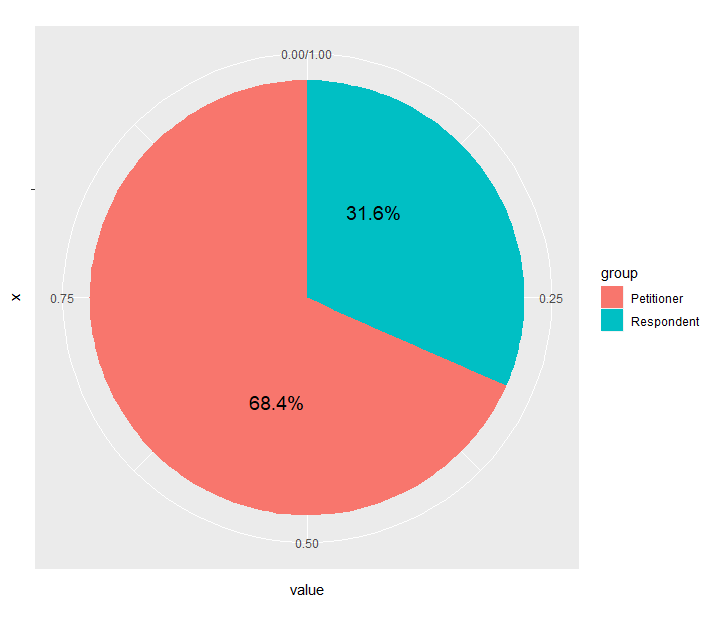
\includegraphics[width=7cm]{Piechartofcaseoutcomes.png}
\end{column}
\begin{column}{.4\textwidth}
One interesting point is that Petitioners are far more likely to succeed in this sample than Respondents. This is consistent with the "always bet reverse" motto that some legal scholars have taken up.

\end{column}
\end{columns}
\end{frame}

\section{Conclusion}
    \begin{frame}{}
        \vfill
      \centering
      \begin{beamercolorbox}[sep=8pt,center,shadow=true,rounded=true]{title}
        \usebeamerfont{title}\insertsectionhead\par%
        \color{oxfordblue}\noindent\rule{10cm}{1pt} \\
      \end{beamercolorbox}
      \vfill
  \end{frame}
  
\subsection{}
\begin{frame}{Importance of this paper}
\begin{itemize}
\item Practical applications in speech creation tools improving the sentiment profile of speech while they are being written.
\item proof of concept for further research into the usefulness of sentiment analysis in the legal field and possibly other fields that are heavily reliant of persuasive speaking. 
\end{itemize}
\end{frame}

\section{Bibliography}
    \begin{frame}[plain]
        \vfill
      \centering
      \begin{beamercolorbox}[sep=8pt,center,shadow=true,rounded=true]{title}
        \usebeamerfont{title}\insertsectionhead\par%
        \color{oxfordblue}\noindent\rule{10cm}{1pt} \\
      \end{beamercolorbox}
      \vfill
  \end{frame}

\subsection{}
\begingroup
\newcommand\Fontvi{\fontsize{6}{7.2}\selectfont}
\Fontvi

\begin{frame}[plain]

\bibliographystyle{plain}
\bibliography{References}

\end{frame}


\end{document}

